\documentclass[a4paper,14pt]{article}\usepackage{amssymb}\setlength\oddsidemargin{-2cm}\setlength\evensidemargin{-2cm}\setlength\textwidth{17cm}\setlength\topmargin{0cm}\usepackage[dvips]{graphicx}\begin{document}\title{}Number of events: 100
\begin{table}[h] 
\centering\caption{Number of objects per event} 
\begin{tabular}{|c|c|} \hline 
Name & Value\\ \hline 
StsTracks & 2 \\ \hline 
RichRings & 2 \\ \hline 
RichProjections & 1 \\ \hline 
GlobalTracks & 2 \\ \hline 
\end{tabular} \end{table}\begin{table}[h] 
\centering\caption{Number of all, true and fake hits in tracks and rings} 
\begin{tabular}{|c|c|c|c|c|c|} \hline 
 & all & true & fake & true/all & fake/all\\ \hline 
Sts & 7.44 & 7.44 & 0.00498 & 0.999 & 0.000622 \\ \hline 
Rich & 25.77 & 25.42 & 0.343 & 0.987 & 0.0132 \\ \hline 
\end{tabular} \end{table}\begin{table}[h] 
\centering\caption{Number of ghosts per event} 
\begin{tabular}{|c|c|} \hline 
Name & Value\\ \hline 
Sts & 0 \\ \hline 
StsRichMatching & 0 \\ \hline 
Rich & 0 \\ \hline 
Rich & 0 \\ \hline 
RichStsMatching & 0 \\ \hline 
RichElId & 0 \\ \hline 
\end{tabular} \end{table}\begin{table}[h] 
\centering\caption{Tracking efficiency} 
\begin{tabular}{|c|c|} \hline 
 & Electron\\ \hline 
Sts (Sts) & 100(2/2) \\ \hline 
\end{tabular} \end{table}\begin{table}[h] 
\centering\caption{Tracking efficiency} 
\begin{tabular}{|c|c|} \hline 
 & Electron\\ \hline 
Sts (StsRich) & 100(2/2) \\ \hline 
StsRich (StsRich) & 98.5(1.9/2) \\ \hline 
\end{tabular} \end{table}\begin{table}[h] 
\centering\caption{Tracking efficiency} 
\begin{tabular}{|c|c|c|} \hline 
 & Electron & All\\ \hline 
Sts (Sts) & 100(2/2) & 99.5(2/2) \\ \hline 
\end{tabular} \end{table}\begin{table}[h] 
\centering\caption{Tracking efficiency} 
\begin{tabular}{|c|c|c|} \hline 
 & Electron & ElectronReference\\ \hline 
Sts (StsRich) & 100(2/2) & 100(2/2) \\ \hline 
StsRich (StsRich) & 99(1.9/2) & 99(1.9/2) \\ \hline 
Rich (Rich) & 100(2/2) & 100(2/2) \\ \hline 
\end{tabular} \end{table}\begin{table}[h] 
\centering\caption{Pion suppression} 
\begin{tabular}{|c|c|} \hline 
 & Pion suppression\\ \hline 
Rich - WrongMatch & 0 (0/0) \\ \hline 
Rich - TrueMatch & 0 (0/0) \\ \hline 
Rich - All & 0 (0/0) \\ \hline 
\end{tabular} \end{table}\begin{figure}[h]
\centering
\includegraphics[width=7cm]{png/tracking_qa_global_tracking_efficiency_all_Sts_p.eps}
\caption{tracking_qa_global_tracking_efficiency_all_Sts_p}
\end{figure}
\begin{figure}[h]
\centering
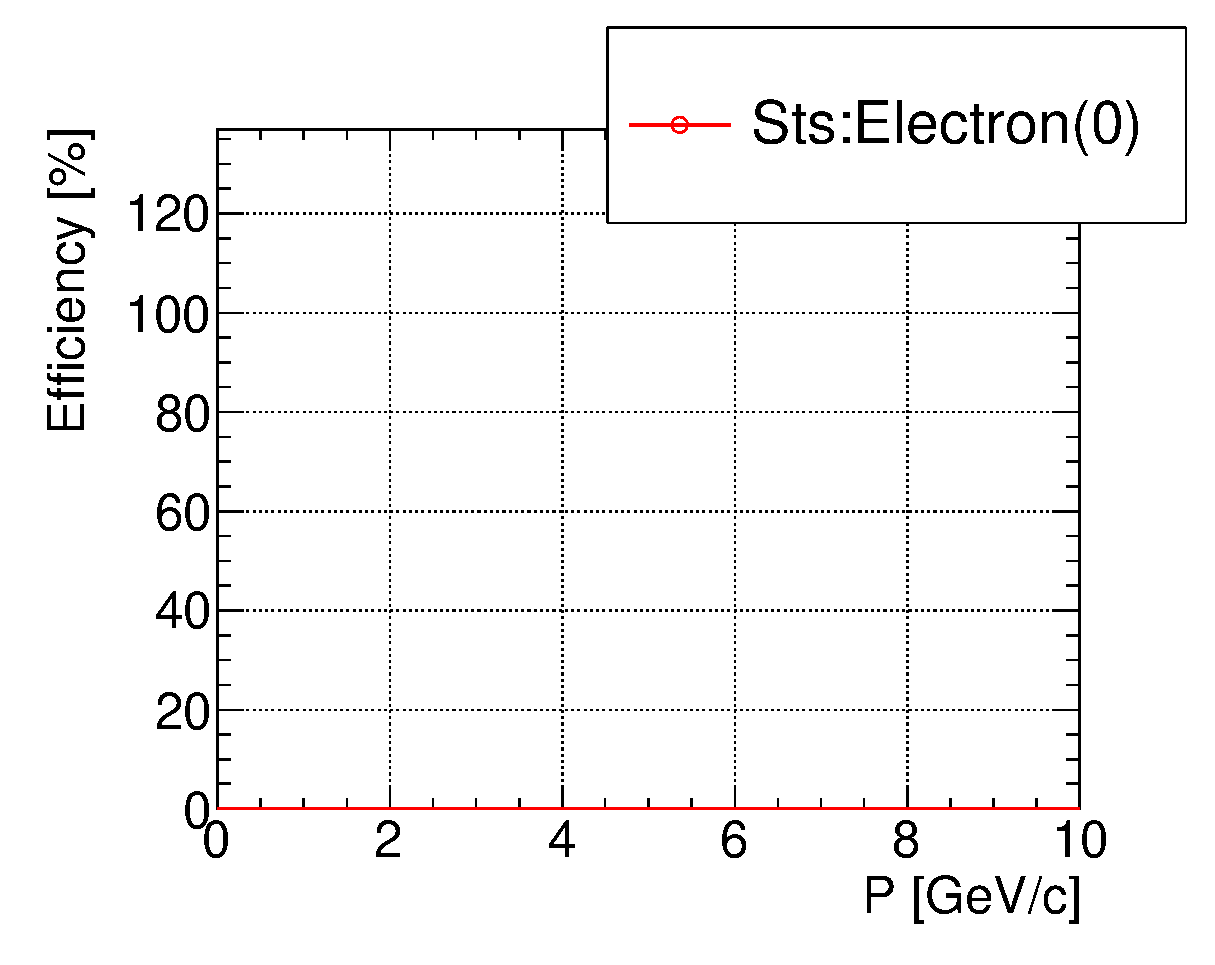
\includegraphics[width=7cm]{png/tracking_qa_global_tracking_efficiency_electron_Sts_p.eps}
\caption{tracking_qa_global_tracking_efficiency_electron_Sts_p}
\end{figure}
\begin{figure}[h]
\centering
\includegraphics[width=7cm]{png/tracking_qa_global_tracking_efficiency_Sts_angle.eps}
\caption{tracking_qa_global_tracking_efficiency_Sts_angle}
\end{figure}
\begin{figure}[h]
\centering
\includegraphics[width=7cm]{png/tracking_qa_global_tracking_efficiency_electron_StsRich_p.eps}
\caption{tracking_qa_global_tracking_efficiency_electron_StsRich_p}
\end{figure}
\begin{figure}[h]
\centering
\includegraphics[width=7cm]{png/tracking_qa_pid_efficiency_electron_StsRich_p.eps}
\caption{tracking_qa_pid_efficiency_electron_StsRich_p}
\end{figure}
\begin{figure}[h]
\centering
\includegraphics[width=7cm]{png/tracking_qa_local_tracking_efficiency_Sts_p.eps}
\caption{tracking_qa_local_tracking_efficiency_Sts_p}
\end{figure}
\begin{figure}[h]
\centering
\includegraphics[width=7cm]{png/tracking_qa_local_tracking_efficiency_Sts_angle.eps}
\caption{tracking_qa_local_tracking_efficiency_Sts_angle}
\end{figure}
\begin{figure}[h]
\centering
\includegraphics[width=7cm]{png/tracking_qa_local_tracking_efficiency_Rich_p.eps}
\caption{tracking_qa_local_tracking_efficiency_Rich_p}
\end{figure}
\begin{figure}[h]
\centering
\includegraphics[width=7cm]{png/tracking_qa_local_tracking_efficiency_Rich_RingNh.eps}
\caption{tracking_qa_local_tracking_efficiency_Rich_RingNh}
\end{figure}
\begin{figure}[h]
\centering
\includegraphics[width=7cm]{png/tracking_qa_local_tracking_efficiency_Rich_BoA.eps}
\caption{tracking_qa_local_tracking_efficiency_Rich_BoA}
\end{figure}
\begin{figure}[h]
\centering
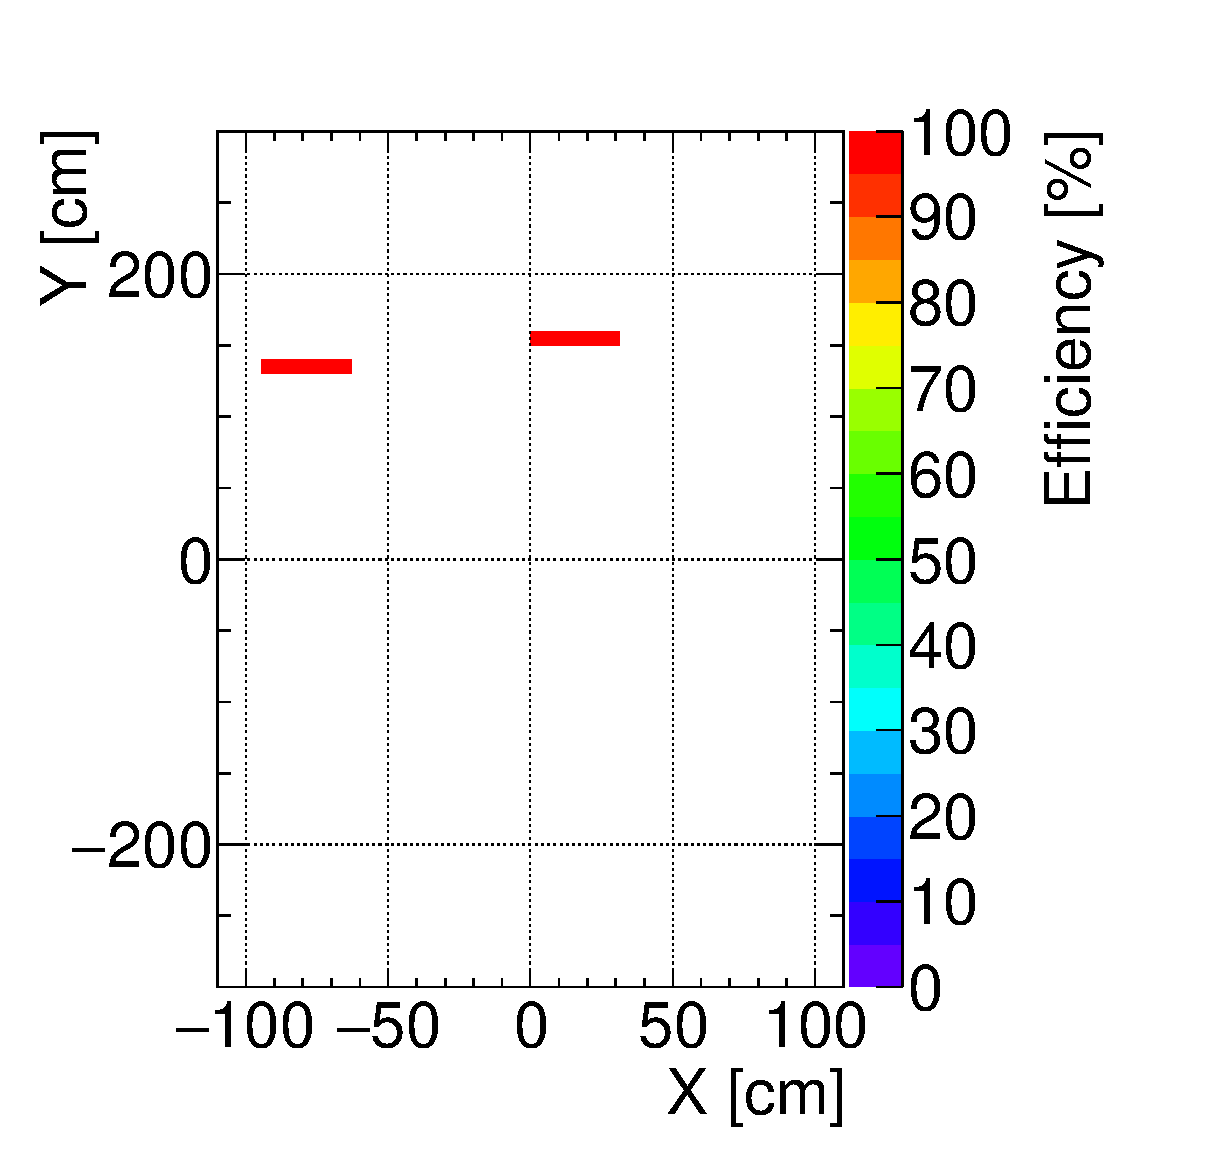
\includegraphics[width=7cm]{png/tracking_qa_Rich_Rich_Electron_Eff_RingXcYc.eps}
\caption{tracking_qa_Rich_Rich_Electron_Eff_RingXcYc}
\end{figure}
\begin{figure}[h]
\centering
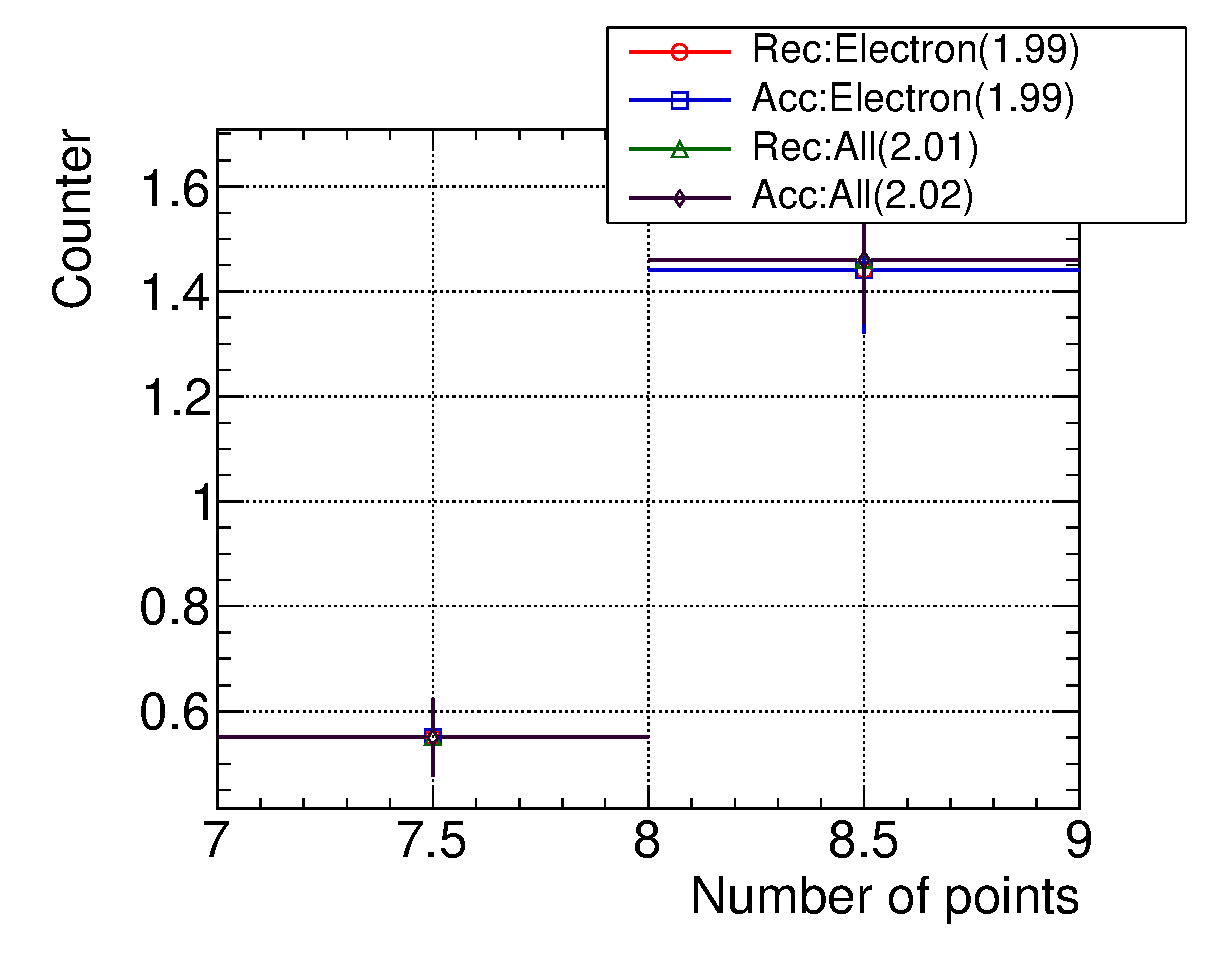
\includegraphics[width=7cm]{png/tracking_qa_local_acc_and_rec_Sts_Np.eps}
\caption{tracking_qa_local_acc_and_rec_Sts_Np}
\end{figure}
\begin{figure}[h]
\centering
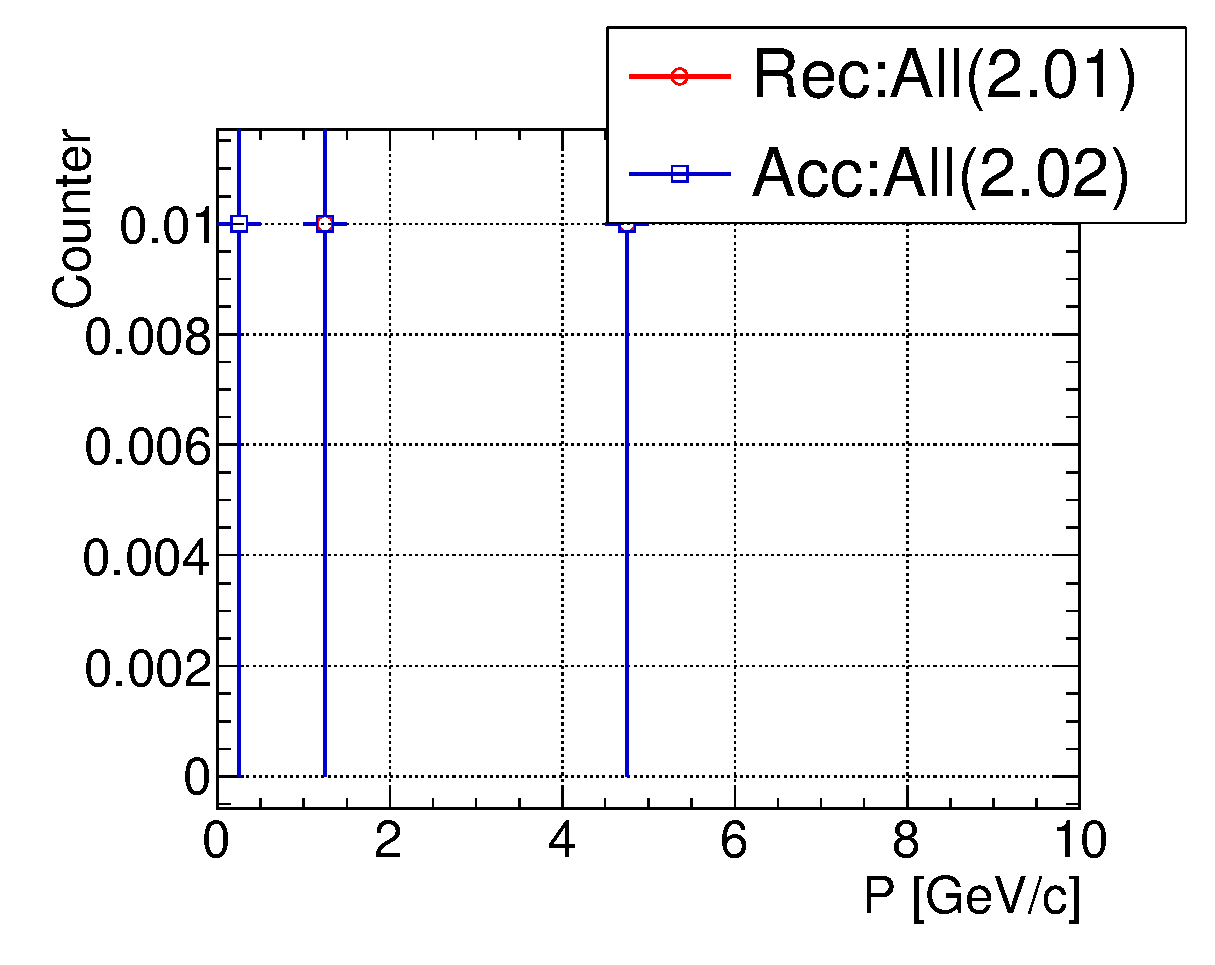
\includegraphics[width=7cm]{png/tracking_qa_local_acc_and_rec_Sts_All_p.eps}
\caption{tracking_qa_local_acc_and_rec_Sts_All_p}
\end{figure}
\begin{figure}[h]
\centering
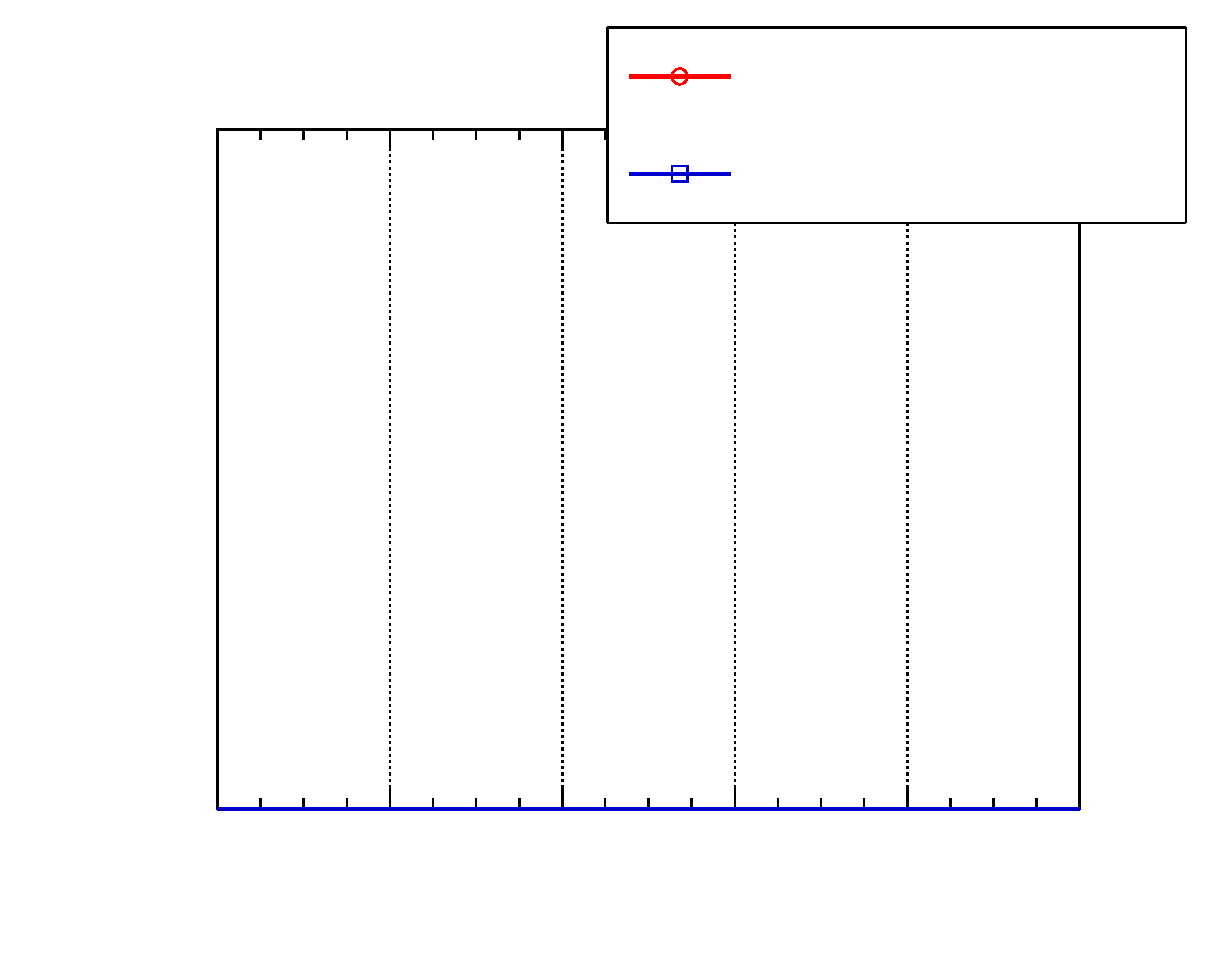
\includegraphics[width=7cm]{png/tracking_qa_local_acc_and_rec_Sts_ElectronMuon_p.eps}
\caption{tracking_qa_local_acc_and_rec_Sts_ElectronMuon_p}
\end{figure}
\begin{figure}[h]
\centering
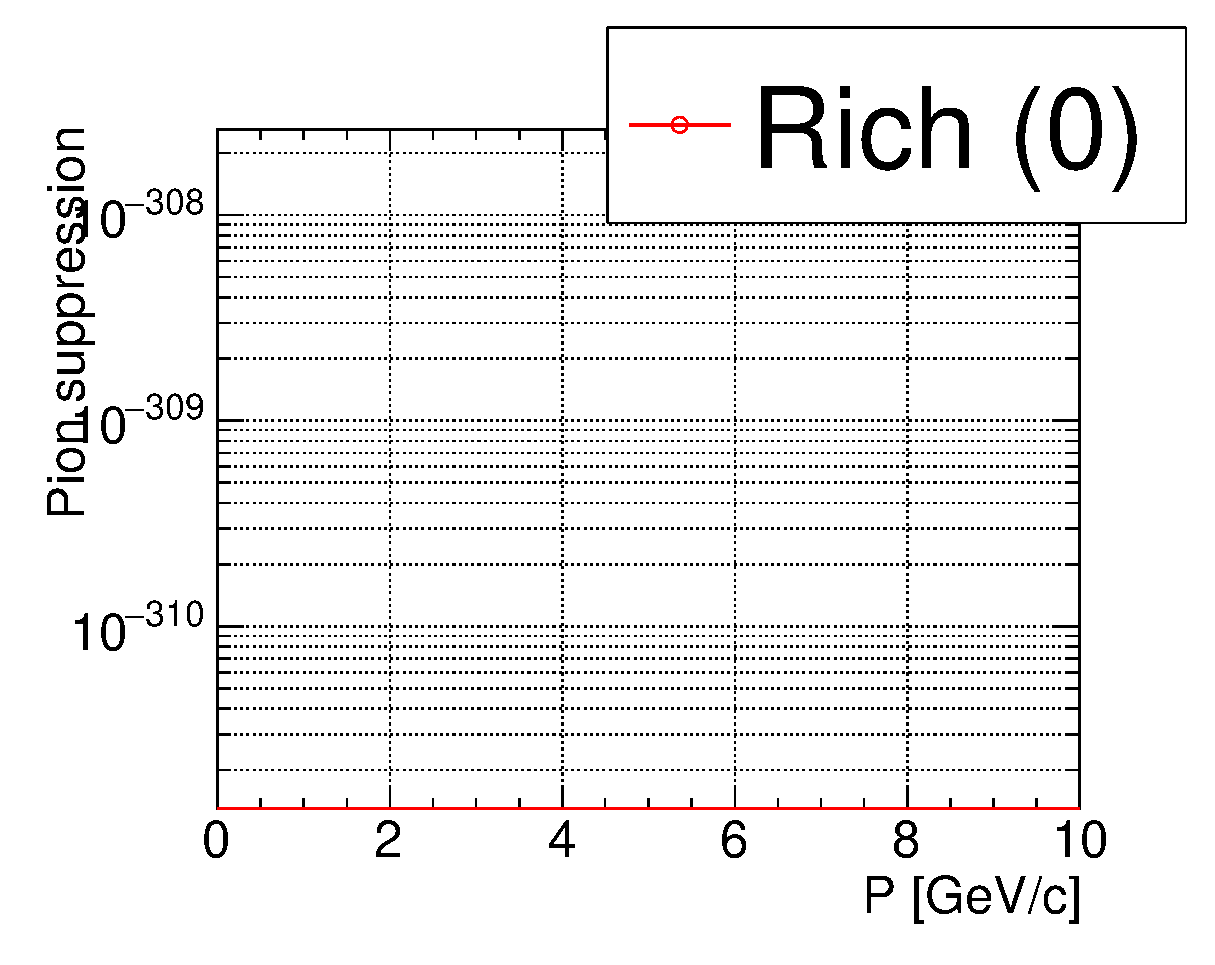
\includegraphics[width=7cm]{png/tracking_qa_pion_suppression_with_rich_p.eps}
\caption{tracking_qa_pion_suppression_with_rich_p}
\end{figure}
\begin{figure}[h]
\centering
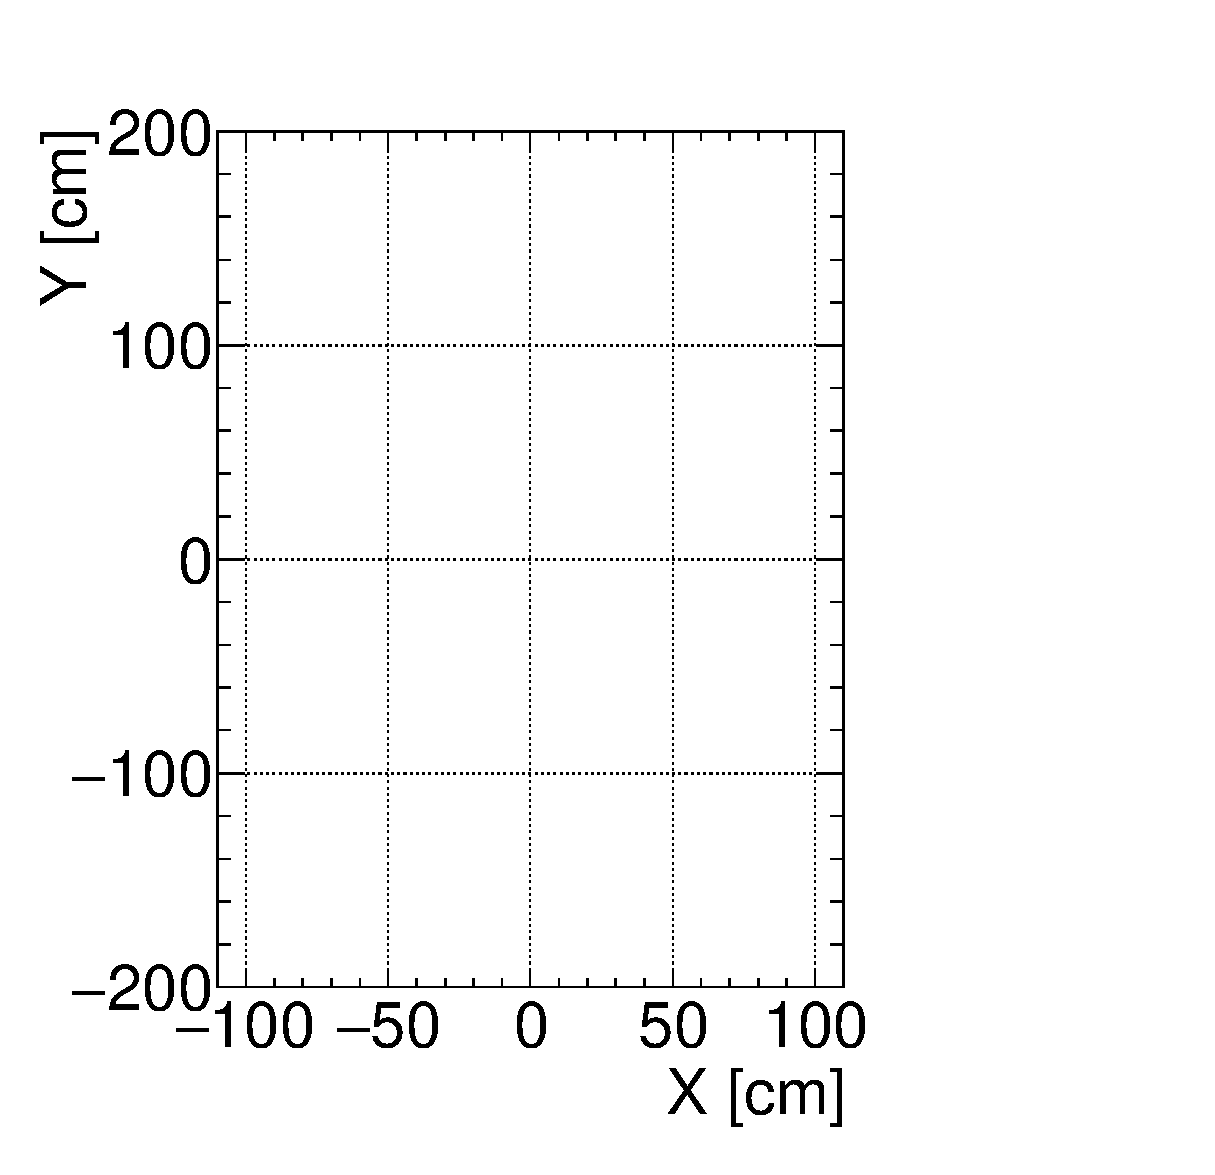
\includegraphics[width=7cm]{png/tracking_qa_hng_NofGhosts_Rich_RingXcYc.eps}
\caption{tracking_qa_hng_NofGhosts_Rich_RingXcYc}
\end{figure}
\begin{figure}[h]
\centering
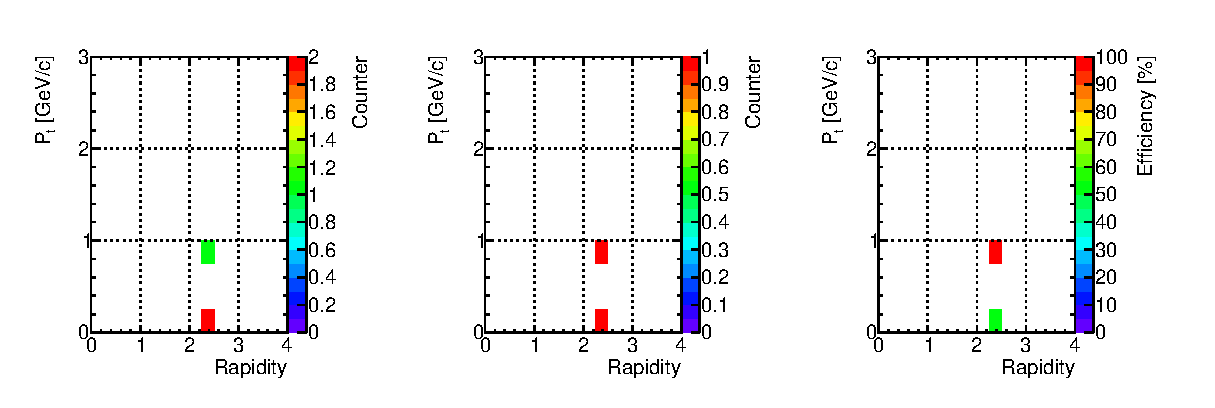
\includegraphics[width=7cm]{png/tracking_qa_Sts_all_ypt.eps}
\caption{tracking_qa_Sts_all_ypt}
\end{figure}
\begin{figure}[h]
\centering
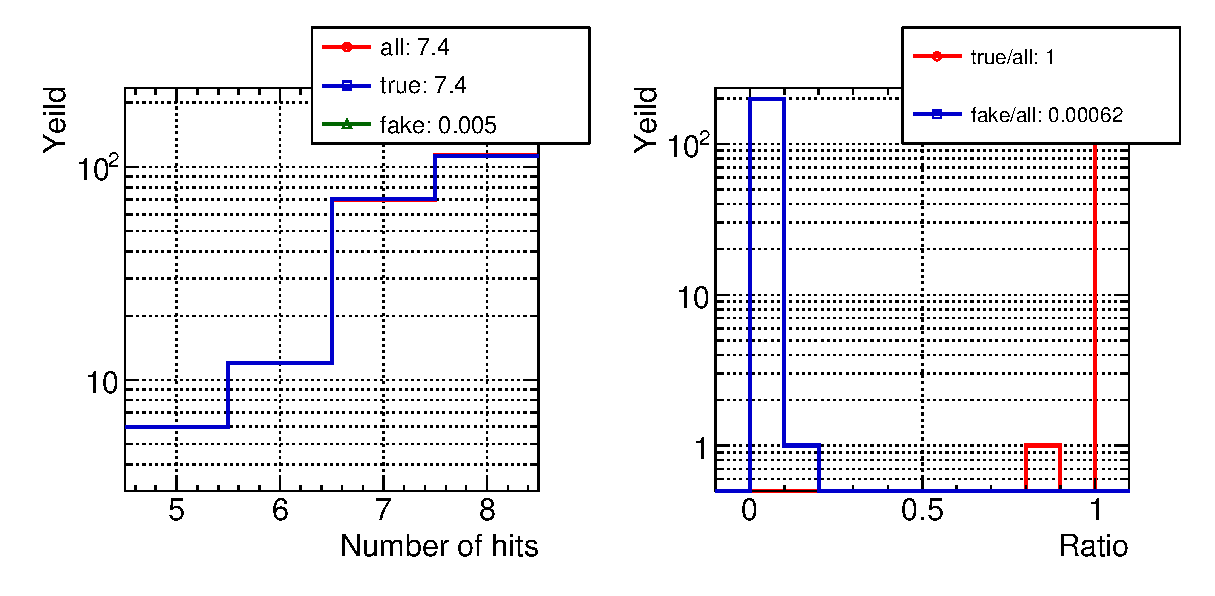
\includegraphics[width=7cm]{png/tracking_qa_sts_hits.eps}
\caption{tracking_qa_sts_hits}
\end{figure}
\begin{figure}[h]
\centering
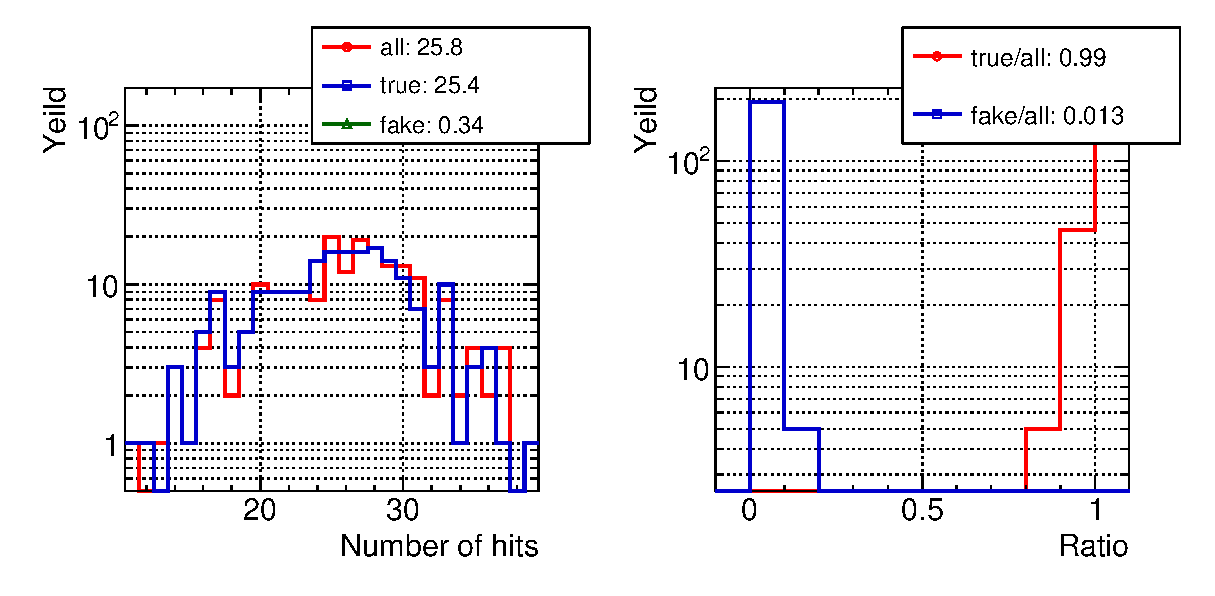
\includegraphics[width=7cm]{png/tracking_qa_rich_hits.eps}
\caption{tracking_qa_rich_hits}
\end{figure}
\end{document}